\chapter{Testy systemu}
\label{sec:tests}
W tym rozdziale przedstawione są różne konfiguracje pakietów, wraz z wykresami ruchów platform, oraz wnioski płynące z tych zachowań.
Każdy test wymaga innego podłączenia komponentów do siebie nawzajem.

Wyniki pomiarów zostały zebrane za pomocą ROSowego narzędzia \texttt{rosbag}, a następnie wyeksportowane do pliku CSV. Za pomocą programu Gnuplot narysowano wykresy.

\section{Testy robota}
	Platforma została przetestowana na trasie kwadratu w identyczny sposób, jak w eksperymencie poniżej.
	To dało dokładne informacje o zachowaniu się czujników urządzenia, jak i o wielkości błędów.

\section{Porównanie modeli dynamiki i kinematyki}
	Posiadając model kinematyczny, którego ruch jest sterowany wzorami, można porównać jego pozycję i rotację z modelem dynamicznym.
	Należy w tym samym momencie nadać bazom identyczne prędkości kół i zebrać dane dotyczące wzajemnej pozycji.
	Modele rozpoczynają jazdę z punktu (0,0), początkowo stoją 5 s w miejscu, aż symulator i wszystkie komponenty się załączą.
	
	Te eksperymenty pozwalają sprawdzić, jak model dynamiczny zachowuje się w stosunku do idealnego modelu kinematycznego.
	
	\begin{figure}[H]
		\centering
		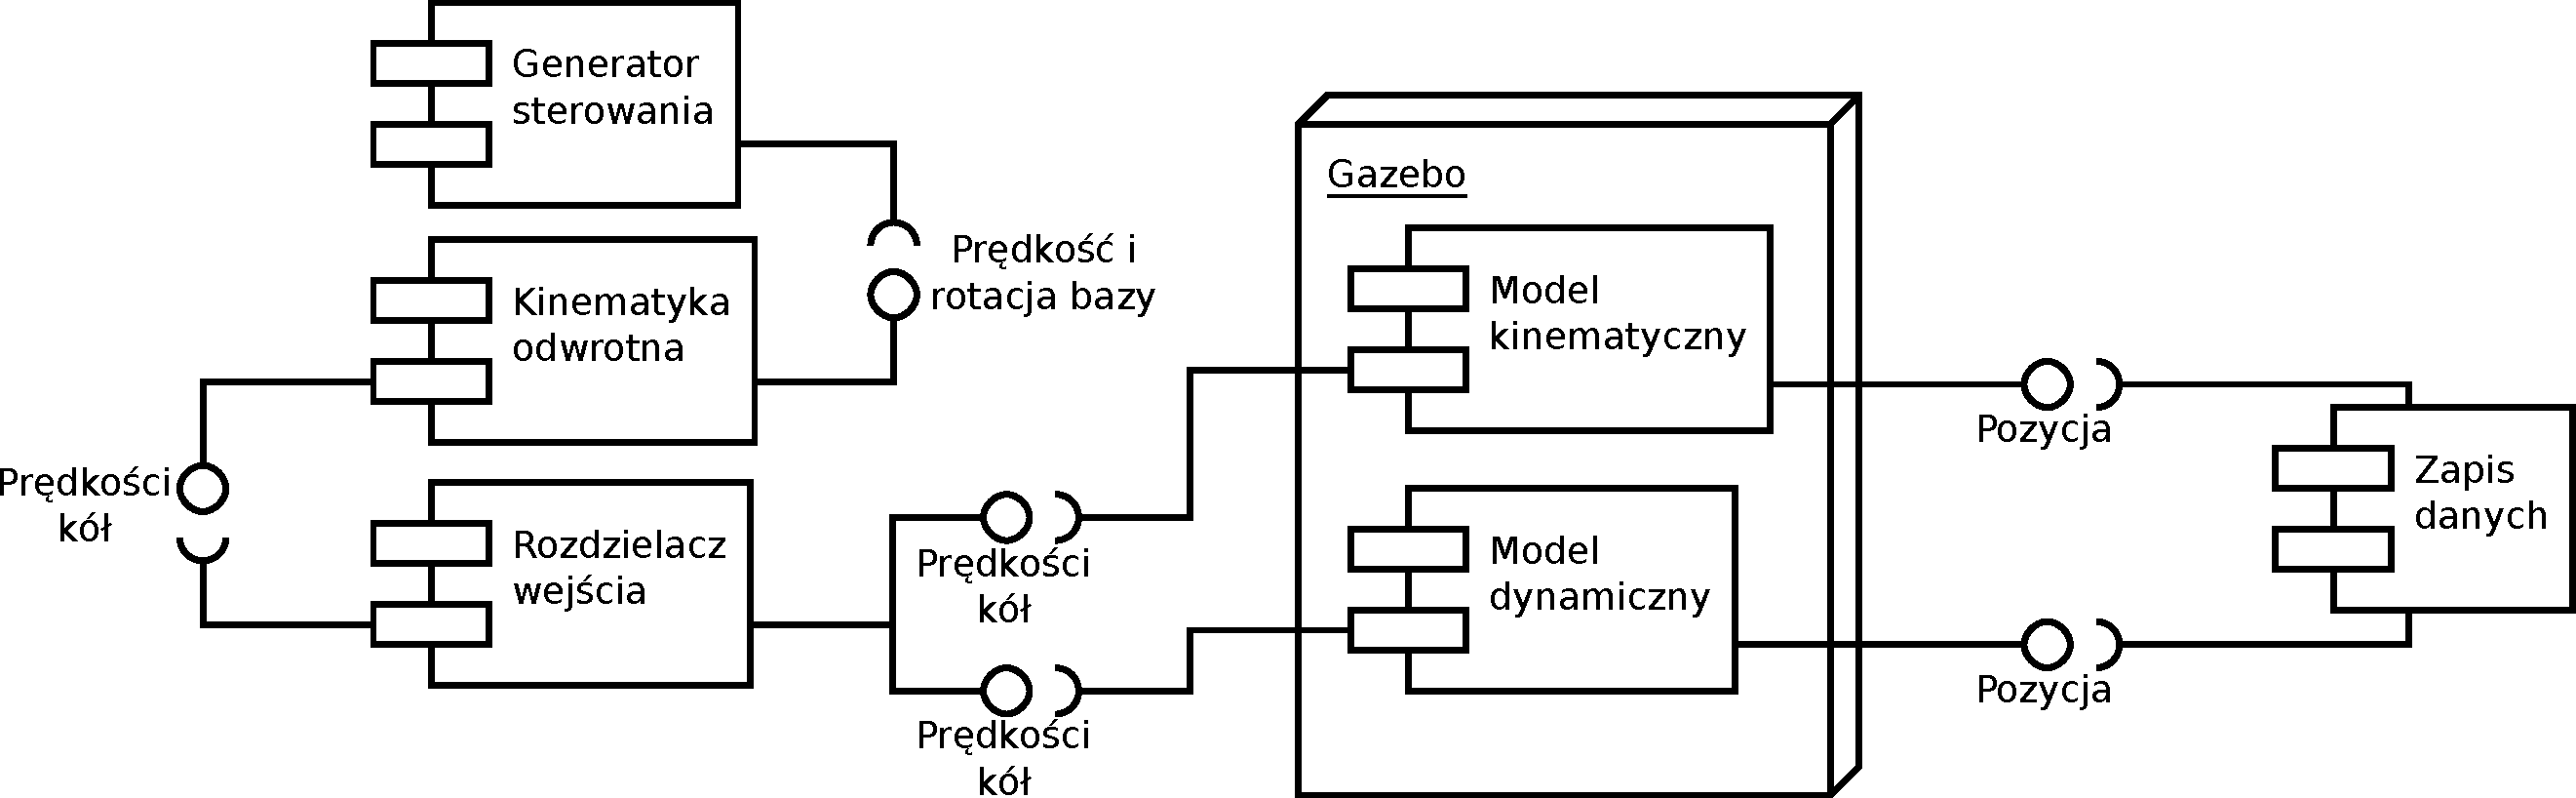
\includegraphics[width=\textwidth]{uml/gramofon.pdf}
			\caption{Połączenie komponentów w celu przetestowania wzajemnego ruchu modelu kinematycznego i dynamicznego.}
		\label{uml:gramofon}
	\end{figure}
	
	\subsection{Ruch po kwadracie}
		\label{sec:test_square}
		Wywołano ruch z prędkością 0,2 $\frac{m}{s}$ po kwadracie o boku 1 m, bez nadawania prędkości kątowej.
		Modele przejechały ścieżkę pięciokrotnie, po czym zatrzymały się. W kątach kwadratu nie było nadania prędkości zerowej.
		
		Celem tego eksperymentu było sprawdzenie, czy model dynamiczny będzie wykazywał odchylenia w trakcie jazdy po prostej ścieżce 
		i jak będzie reagował na nagłe zmiany kierunku jazdy.
		
		\begin{figure}[H]
			\centering
			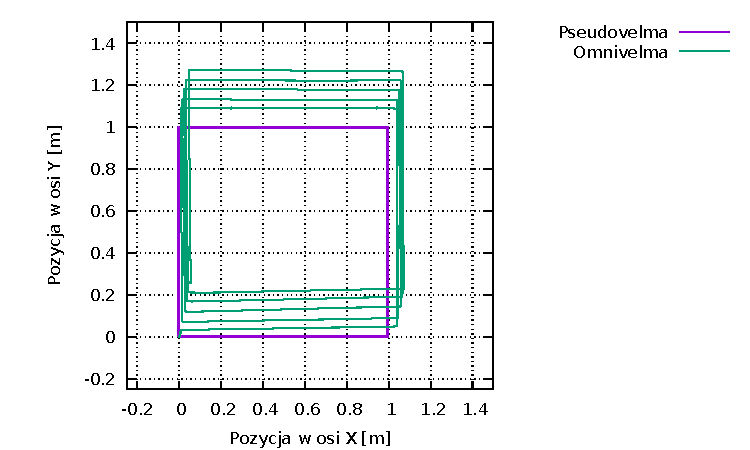
\includegraphics[width=\textwidth]{plots/square.pdf}
				\caption{Ruch modelu kinematycznego i dynamicznego po kwadratowej ścieżce.}
			\label{plot:gramofon_square}
		\end{figure}
		
		Po pierwsze widać, że tuż przed rozpoczęciem jazdy model dynamiczny odsunął się o kilka centymetrów od pozycji początkowej i obrócił nieznacznie.
		Jest to spowodowane tym, że maszyna do symulacji fizyki działa na liczbach zmiennoprzecinkowych pojedynczej precyzji,
		zatem nie wszystkie siły działające na obiekty będą się dokładnie równoważyć i może istnieć mały ruch w losowych kierunkach i rotacja.
		
		Następnie, po nadaniu ruchu w bok, platformy jechały po linii prostej.
		Model dynamiczny wykonał większą trasę do modelu kinematycznego, co nie jest spowodowane poślizgiem.
		Na takie zachowanie wpływa wiele czynników, zarówno wewnętrzna implementacja maszyny symulacyjnej fizyki, jak i natura użytych algorytmów.
		
		Przy zmianie prędkości widać poślizg przy zatrzymywaniu się z danego kierunku.
		Kąty trasy są zaokrąglone w jednym kierunku, co pokazuje że model dynamiczny posiada bezwładność. 
		Gdy otrzymuje nowe prędkości kół, nadal porusza się jeszcze przez pewien czas w poprzednim kierunku.
		Poślizg przy ruszaniu jest mniejszy.
		To zjawisko nie wpływa istotnie na trasę modelu, gdyż przy testach, w których prędkość zmieniała się wolno i w których nie występowały nagłe hamowania,
		nadal występowało takie samo zboczenie w stosunku do trasy kinematycznej.
		
		Testy platformy pokazały, że robot w rzeczywistości zachowuje się bardzo podobnie, również występują takie poślizgi przy nagłej zmianie kierunku prędkości.
		
		Za każdym obiegiem pętli narasta różnica pozycji wynikającej z kinematyki i pozycji obliczonej przez symulator.
		Po zatrzymaniu się modelu dynamicznego, ponownie porusza się on jeszcze przez pewien czas w losowym kierunku, innym niż na początku,
		aż do przerwania testu.
	
	\subsection{Ruch po ,,rozecie''}
		Drugi, bardziej skomplikowany test składa się na ruchy platform w przód i w tył, oraz obrót wokół punktu.
		
		Modele jechały 2 m w przód z prędkością 0,25 $\frac{m}{s}$, następnie następował obrót o 45°, po czym odbywała się jazda w tył.
		Na koniec ruch w bok przy jednoczesnym obrocie i powtórzenie cyklu. Czterokrotne wykonanie tego zamyka trasę.
		
		\begin{figure}[H]
			\centering
			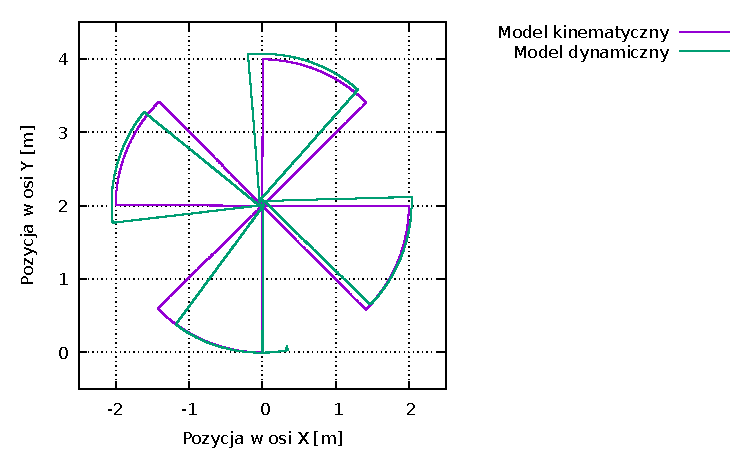
\includegraphics[width=\textwidth]{plots/sun.pdf}
				\caption{Ruch modelu kinematycznego i dynamicznego po rozetowej ścieżce.}
			\label{plot:gramofon_sun}
		\end{figure}
		
		Z wykresu wywnioskować można, prócz tego co z poprzedniego eksperymentu, to że model dynamiczny przegania model kinematyczny również w kwestii obrotu.
		W tym przypadku składowa trasy pionowej (w lokalnym układzie), czyli prędkość w przód i w tył, zniosła się.
		Obrót i ruch w bok były ciągle narastające, a co za tym idzie, spowodowały przesunięcie się modelu dynamicznego, co widać, porównując ich końcową pozycję.
		
	\subsection{Powtarzalność testów}
		Pomimo, że na środowisko wirtualne w maszynie symulacyjnej fizyki nie działają żadne zjawiska zewnętrzne, nadal jej działanie zależy od wewnętrznych niedoskonałości
		systemu, na którym działa. W to wchodzą takie rzeczy, jak niedokładności w reprezentacji liczb zmiennoprzecinkowych, czas pomiędzy kolejnymi klatkami symulacji i 
		niedeterministyczne przekazywanie wiadomości przez system operacyjny.
		
		Zatem każdy test będzie generował nieco inne wyniki pozycji modelu zarówno kinematycznego, jak i dynamicznego. 
		Jednak w kinematycznym przypadku różnice są niezauważalne.
		Przeprowadzono powyższe testy trzykrotnie, aby zbadać jak bardzo każdy z przejazdów modelu różni się od poprzedniego.
		
		\begin{figure}[H]
			\centering
			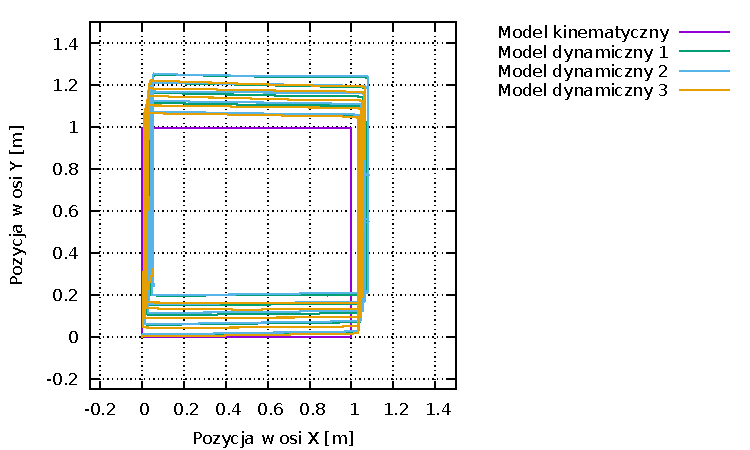
\includegraphics[width=\textwidth]{plots/square_3.pdf}
				\caption{Wielokrotny ruch modelu kinematycznego i dynamicznego po kwadratowej ścieżce.}
			\label{plot:gramofon_square_3}
		\end{figure}
		
		\begin{figure}[H]
			\centering
			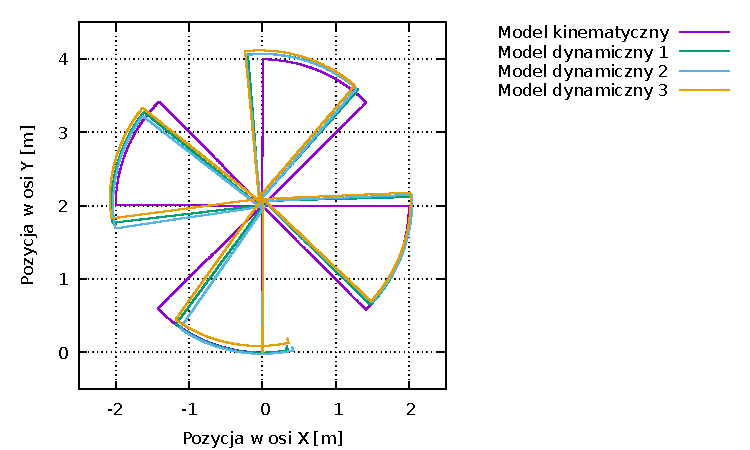
\includegraphics[width=\textwidth]{plots/sun_3.pdf}
				\caption{Wielokrotny ruch modelu kinematycznego i dynamicznego po rozetowej ścieżce.}
			\label{plot:gramofon_sun_3}
		\end{figure}
		
		Wygląda to tak, że odległość pomiędzy pozycjami modelu dynamicznego w różnych testach zwiększa się w czasie.
		Różnica narasta wraz z pokonaną odległością.
		Takie zjawisko jest typowe dla symulacji w których istnieje wiele czynników zewnętrznych, wpływających na symulację.
		
		Aby zmniejszyć te niedoskonałości, należałoby, po pierwsze uruchomić symulację na systemie czasu rzeczywistego, a po drugie zwiększyć 
		dokładność reprezentacji liczb zmiennoprzecinkowych, a co za tym idzie, znacząco zwiększyć obciążenie procesora.
		
		Nie można nadal pozwolić na to, aby symulacja przestała odbywać się w czasie rzeczywistym, gdyż to spowodowałoby opóźnienia w ruchu platform.
		Ponieważ, na przykład, jeśli program sterujący wywoła przez sekundę ruch z prędkością 1 $\frac{m}{s}$, aby przejechać dystans 1 m,
		a obciążony symulator będzie nadawał tą prędkość przez ten czas, to w stosunku od obciążenia, może być to inny czas symulacji.
		Zatem patrząc z perspektywy modelu, sterowanie platformie nadawane będzie przez krótszy czas, niż zakłada to program sterujący i model przejedzie mniejszą odległość.
		Należałoby buforować wszystkie otrzymywane wiadomości i stosować je dopiero w czasie symulacji zgodnym z czasem odebrania pakietu. 
		Ale tutaj także jest problem z generowaniem danych, nawet jeśli wygenerowane dane opatrzone będą nagłówkiem z czasem symulatora, to i tak program obierający będzie miał
		problem z zastosowaniem ich. Dochodzi do problemu synchronizacji programu sterującego i symulatora w niestałym czasie. 
		Wymagałoby to stosowania marszczenia czasu i podobnych technik.
		
\section{Enkodery}
	Model czujnika enkoderów zwraca aktualną prędkość i pozycję kół modelu dynamicznego.
	W ten sposób jest możliwe dokładniejsze określenie pozycji platformy, niż bazując na modelu kinematycznym.
	Jednakże, ta metoda także ma swoje ograniczenia, ze względu na poślizgi, zatem program sterujący nie może w pełni bazować na tych czujnikach, a jedynie powinien używać ich pomocniczo.
	
	Ten test ma za zadanie sprawdzić, czy gdyby poruszać platformą kinematyczną tak, jak poruszają się koła platformy dynamicznej, to jak duża była by różnica pomiędzy 
	pozycjami platform.
	
	\begin{figure}[H]
		\centering
		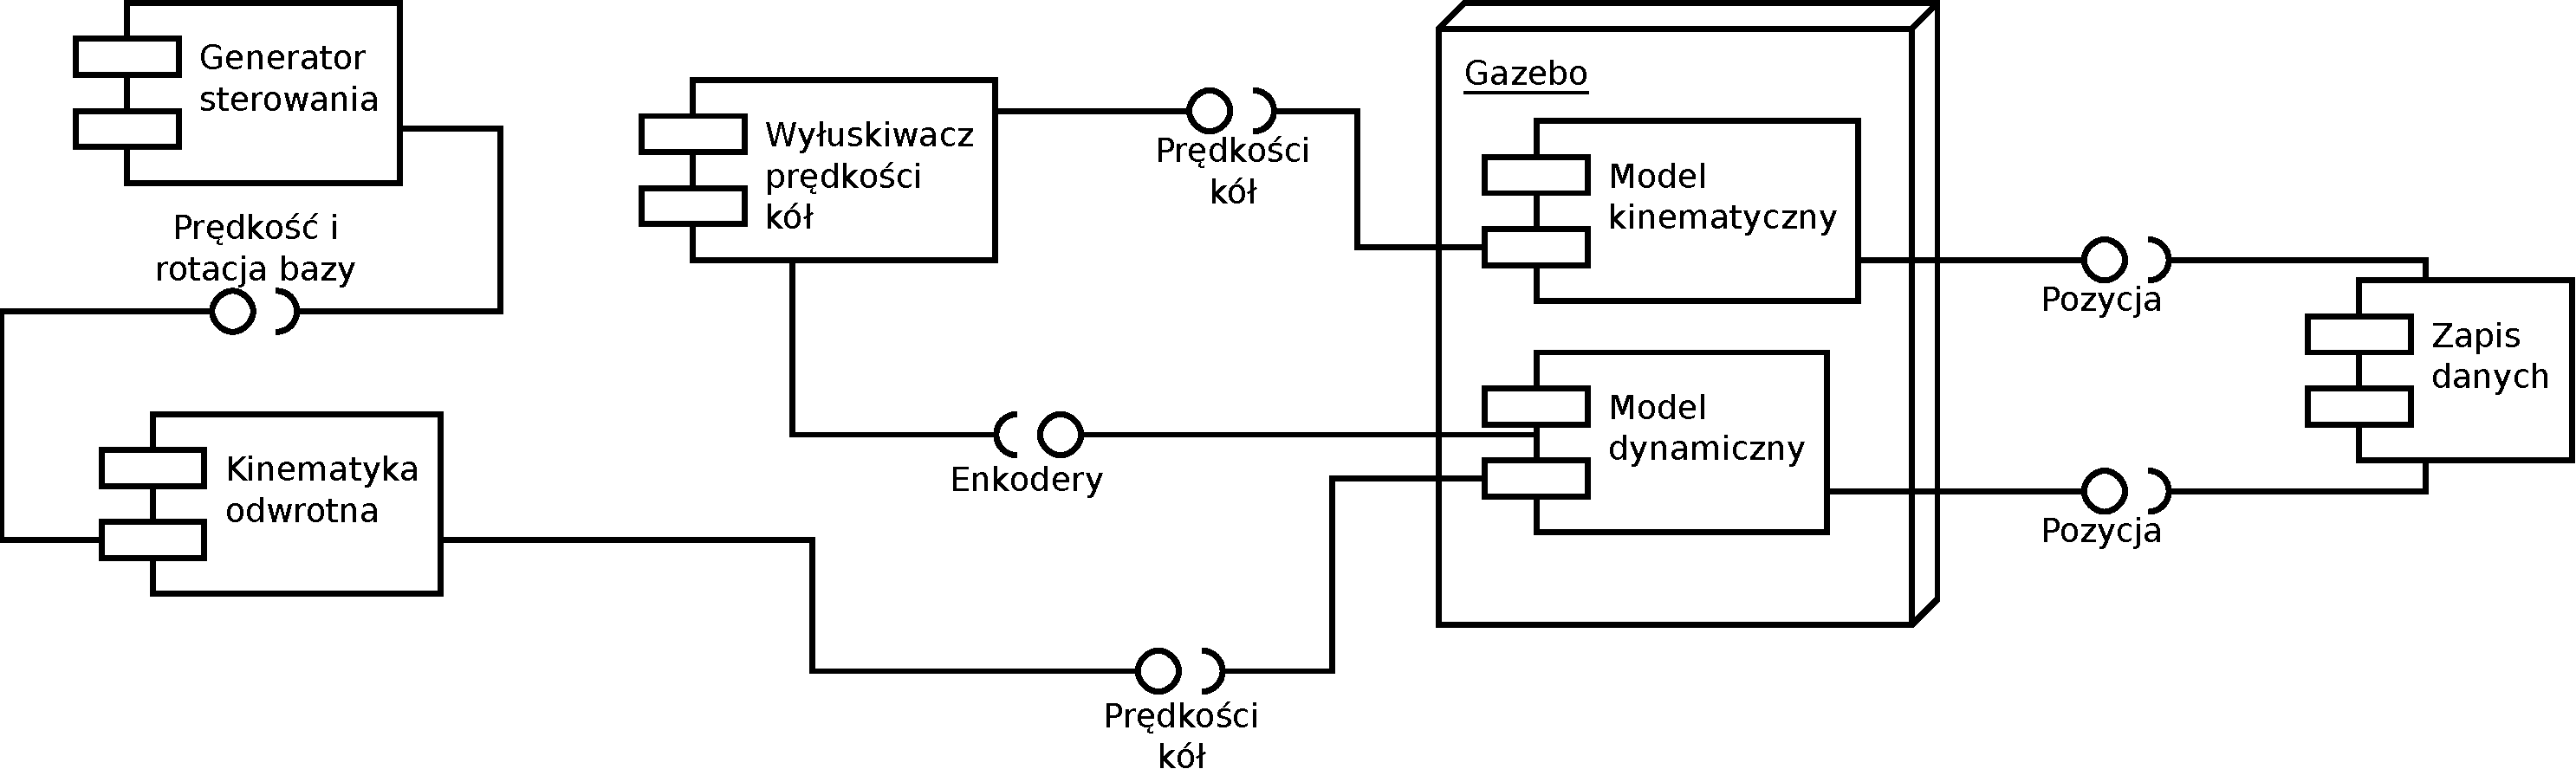
\includegraphics[width=\textwidth]{uml/encoders.pdf}
			\caption{Połączenie komponentów w celu sprawdzenia poprawności działania enkoderów modelu dynamicznego.}
		\label{plot:encoders}
	\end{figure}
	
	Wyjście enkoderów modelu dynamicznego wyłuskane jest z wiadomości i podane dla modelu kinematycznego, model platformy kinematycznej porusza się tak, jak odbiera to model platformy dynamicznej. Nie ma znaczenia bazowy ruch platformy kinematycznej, jednakże pokazany został tutaj dla porównania i uzyskany w taki sposób, jak dla poprzednich testów. 
	
	Przeprowadzono dwa testy, pierwszy standardowy, podobny do powyższych, drugi nadawał prędkości kół jedynie przy zmianie kierunku ruchu modelu dynamicznego.
	Sterowanie zostało stworzone z myślą o wywołaniu poślizgów platformy, nadana prędkość 0,5 $\frac{m}{s}$ była większa, niż w poprzednich testach.
	
	\begin{figure}[H]
		\centering
		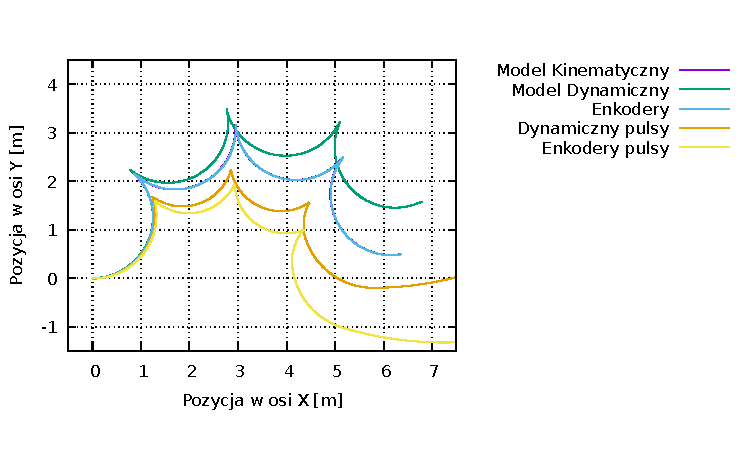
\includegraphics[width=\textwidth]{plots/star_encoders.pdf}
			\caption{Ruch modeli przy ciągłym wysyłaniu pakietów, jedynie na zmiany kierunku i kinematyka bazująca na danych zebranych z enkoderów. Wykres pierwszy i trzeci są na siebie nałożone.}
		\label{plot:star_encoders}
	\end{figure}
	
	\subsection{Ciągłe nadawanie prędkości kół}
		Przy ciągłym nadawaniu prędkości kołom, enkodery odczytują praktycznie dokładnie te same wartości, jakie są nadawane.
		Co za tym idzie, działa to w taki sam sposób, w jaki działałaby platforma kinematyczna w poprzednim teście.
		Pierwsze trzy wykresy zatem nie różnią się przebiegiem, niż gdyby je wygenerować w poprzednim podłączeniu komponentów.
		
		Przy pierwszej zmianie prędkości platformy, widać różnicę w pozycji modeli, spowodowaną poślizgiem.
		Duża prędkość kątowa również powoduje poślizg kątowy, przez co różnica pomiędzy pozycjami w tym samym czasie rośnie szybciej, jak w poprzednich testach.
		Enkodery nie są w stanie wykrywać poślizgu, dlatego ich wykres nie odstaje w momentach zmiany kierunku od wykresu modelu kinematycznego.
		
	\subsection{Impulsowe nadawanie prędkości kół}
		Jedno wywołanie metody maszyny symulacyjnej fizyki nadaje prędkość kołom. Następnie, z powodu symulowanych oporów, prędkość koła naturalnie spada, aż do
		ponownego nadania prędkości. To, jak prędkość ruchu spada, widać, gdyż segmenty przebiegu w dwóch ostatnich wykresach nie są łukami, jak ma to miejsce przy 
		ciągłym nadawaniu prędkości. Po nadaniu ostatniej wiadomości, zatrzymującej wszystkie koła, platforma nadal wolno się porusza, pod wpływem bezwładności, a brak oporu rolek w jednym z kierunków, oraz brak oporu obrotu koła pozwalał na ciągły ruch w losowym kierunku.
		
		Co warto tutaj zauważyć, to to że enkodery prawidłowo starają się przekazać zmienną prędkość kół. 
		Inaczej mówiąc, pozycja wynikająca z danych zwróconych z enkoderów jest dokładniejsza, niż wynikająca z wywołanego ruchu modelu kinematycznego w idealnym przypadku.
		Żółty wykres jest bliżej pomarańczowego, niż fioletowy/niebieski.
		Tutaj także widać wpływ poślizgu modelu na określanie pozycji.
		
		Zatem model enkoderów może mieć faktyczne zastosowanie w określaniu pozycji platformy. 
		Okazuje się lepszy, niż kinematyka, w przypadku zewnętrznego nadania prędkości platformie, na przykład pod wpływem nagłego zatrzymania.
		Pod warunkiem, że nie występuje poślizg. Jak już wcześniej wspomniano, platforma jest podatna na ruch w losowym kierunku przy nagłym zatrzymaniu,
		lecz nie zawsze taki ruch może zostać niewykryty. Poślizg, a nadanie niedeterministycznej siły zewnętrznej, to dwa różne zjawiska.
		
\section{Czujnik inercji}
\label{sec:test_imu}
	Test polega na wymuszeniu określonych prędkości i przyspieszeń na modelu bazy i zebraniu wyników.
	
	\begin{figure}[H]
		\centering
		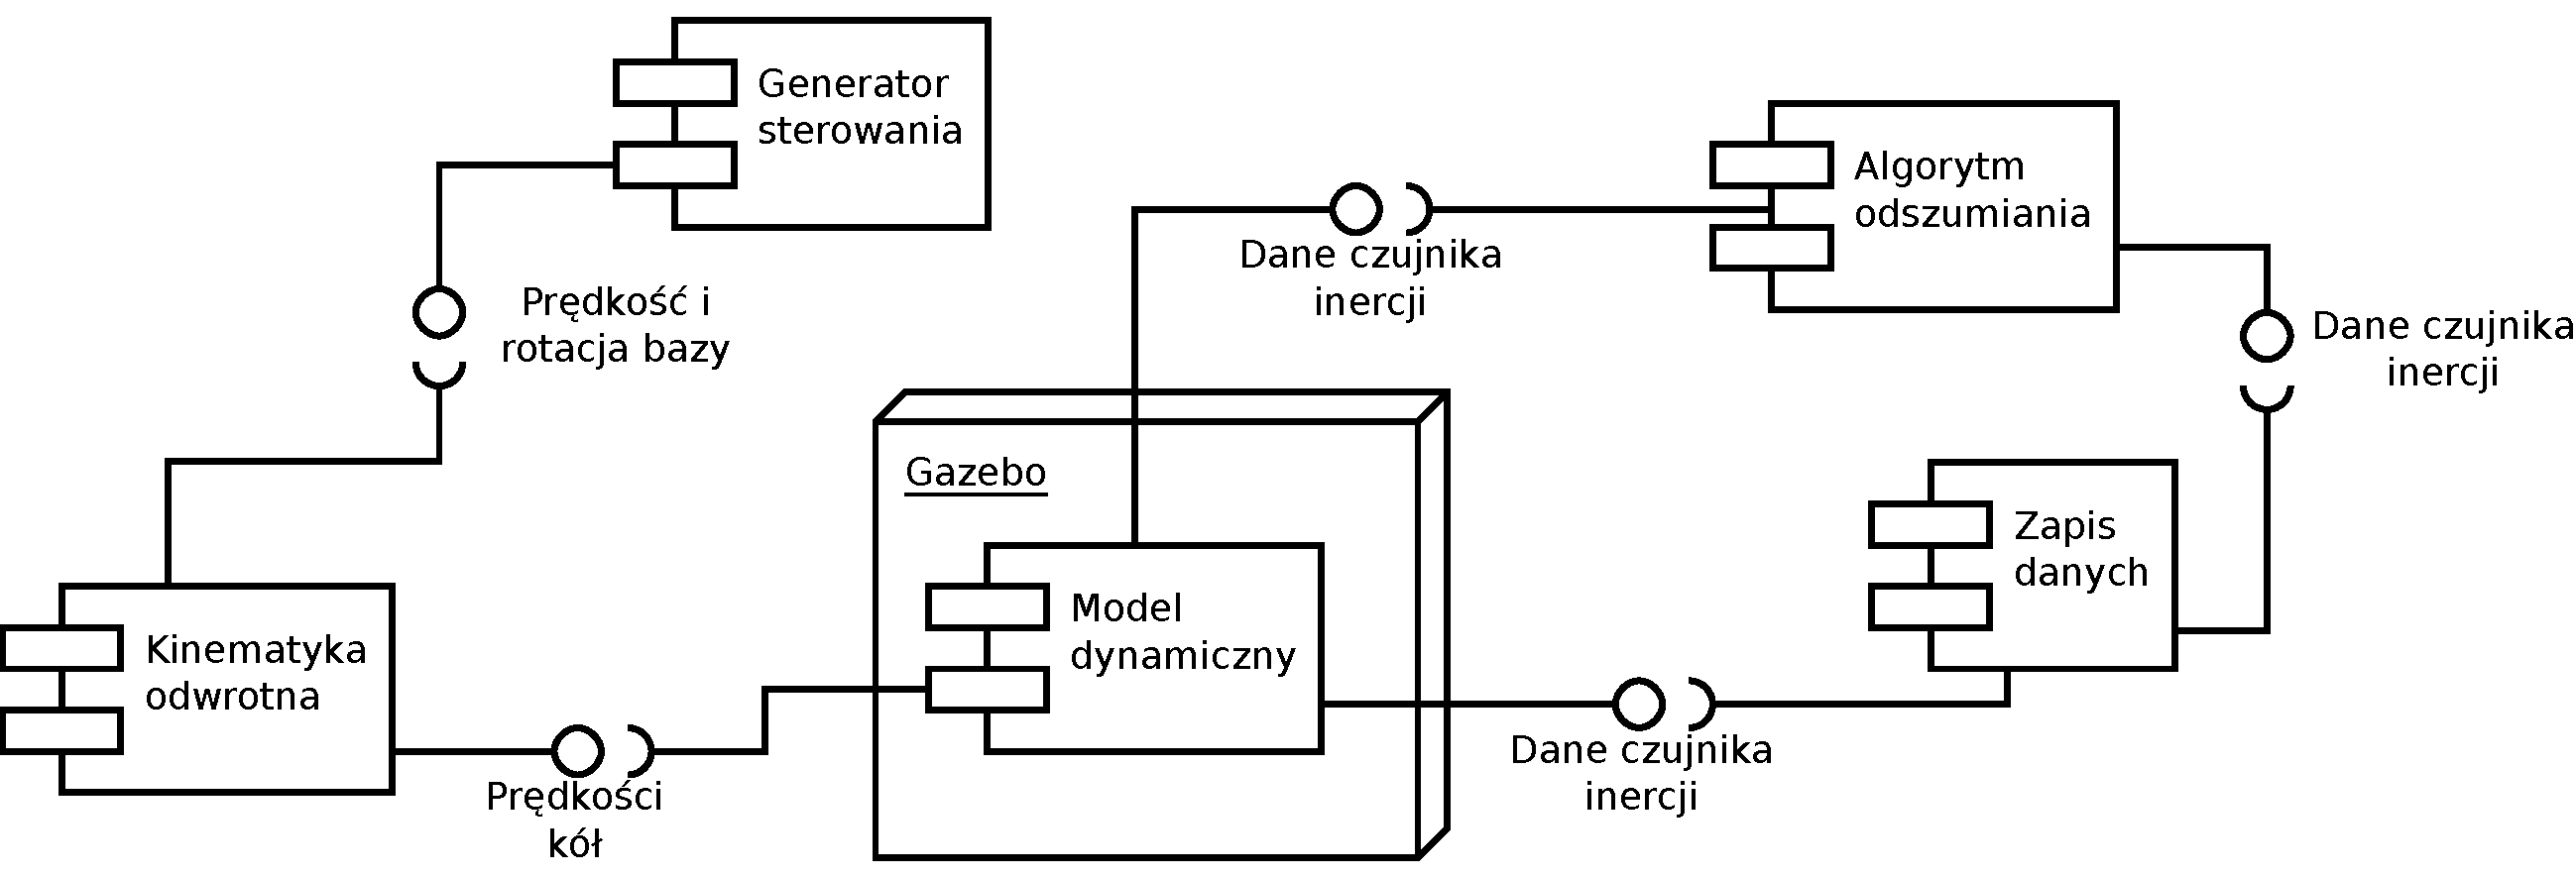
\includegraphics[width=\textwidth]{uml/wewucho.pdf}
		\caption{Połączenie komponentów dla testu czujnika inercji.}
		\label{uml:wewucho}
	\end{figure}
	
	Połączenie nadające sterowanie jest podobne do poprzednich testów.
	Dodatkowy komponent odszumia dane i zapisuje je, aby można je było wygodnie przedstawić na wykresie.
	W tym teście nie jest wymagany model kinematyczny.
	
	\subsection{Czujnik prędkości kątowej}
		Ten czujnik korzysta z żyroskopu i zwraca prędkość kątową we wszystkich trzech osiach.
		Ponieważ jednak platforma porusza się po płaskim terenie, wymagany jest jedynie czujnik w kierunku osi Z, czyli w górę.
		Drugą osią może być zatem czas nadania pakietu.
		
		Wykonano dwa testy, w pierwszym wymuszono ruch po spirali ze stałą prędkością liniową, a co za tym idzie, z nieliniowo zmieniającą się prędkością kątową platformy.
		Prędkość platformy aktualizowana była co 0,5 s, co widać w postaci schodków na wykresie.
		Trasa robota nie pokazywała żadnych nowych zjawisk, które nie zostały już wspomniane w poprzednich testach.
		
		Drugim testem jest ruch po serpentynie.
		Prędkość liniowa platformy była stała, nadawano prędkości kątowe o rosnącej wartości. Model jeździł po łukach o coraz mniejszych promieniach.
		
		Testy rozpoczęły się w tym samym czasie, lecz program nadający sterowanie celowo oczekiwał po rozpoczęciu kilka sekund.
		
		\begin{figure}[H]
		\centering
			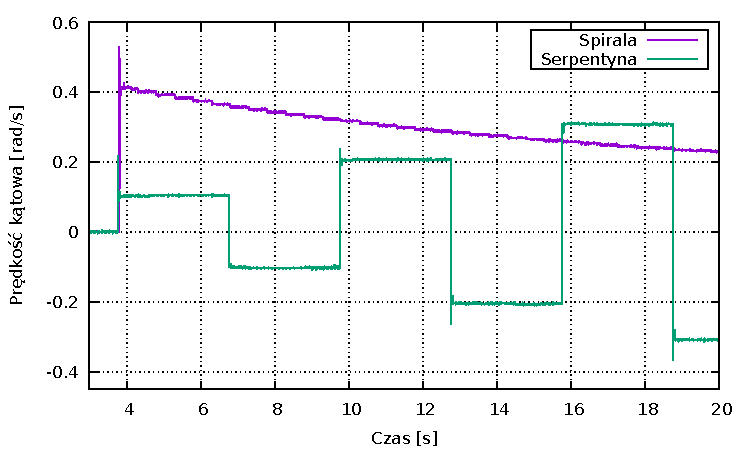
\includegraphics[width=\textwidth]{plots/wewucho_angular.pdf}
			\caption{Test prędkości kątowej czujnika inercji.}
			\label{plot:wewucho_angular}
		\end{figure}
		

		Na początku generowany jest szpikulec, przy natychmiastowym nadaniu prędkości kątowej i liniowej platformie.
		Jest to wewnętrzny szum generowany przez maszynę symulacyjną fizyki, spowodowany dużą zmianą wielu jej parametrów.
		Również wszystkie składowe elementy modelu są symulowane oddzielnie, połączone razem za pomocą więzów.
		Zatem informacja nadająca prędkość platformie przechodzi przez kilka warstw, zanim ustawi odpowiednie prędkości wszystkim składowym systemu.
		
		Widać także niewielką sprężystość modelu, objawia się ona chwilowym zmniejszeniem wartości wielkości tuż po szpikulcu.
		Nie jest to celowo zasymulowana mechanika, a naturalne zjawisko reakcji na akcję. Jeden element składowy platformy działa na drugi, ale za chwilę drugi element także
		zaczyna działać na pierwszy. Podobne jest to w działaniu przeregulowania regulatora.
		
		Jest to zachowanie zbliżone do odczytów z jednostki inercji robota. Tam czujnik również zwraca takie nagłe skoki prędkości w trakcie ruchów.
		Szum w trakcie jednostajnego obrotu jest bardzo podobny.
		
	\subsection{Czujnik przyspieszenia liniowego}
		Jak wcześniej wspomniano, maszyna do symulacji nie posiada wewnętrznie informacji o przyspieszeniu obiektu, gdyż działa w dyskretnych przedziałach czasowych.
		Wartość przyspieszenia musi zostać celowo obliczona, co powodować może różne błędy.
		
		W tym teście platformie nadano przyspieszenie 2 $\frac{m}{s^2}$ przez czas 1 s, w kierunku osi X, w wiadomościach co 0,1 s.
		Następnie platforma poruszała się przez 5 s z prędkością 0,2 $\frac{m}{s}$.
		Potem nadano jej jednoczesne opóźnienie w kierunku osi X i przyspieszenie w kierunku Y, o tych samych wartościach, co na początku.
		Po kolejnych 5 s, platforma zwolniła do zera. Kształt trasy przypominał literę L z zaokrąglonym kątem.
		Samo przyspieszenie platformy wynika z uśrednienia wysyłanych prędkości w czasie, musi być nadawane dyskretnie, żaden z elementów symulatora nie jest w stanie
		pracować w ciągłej domenie czasowej.
		
		\begin{figure}[H]
		\centering
			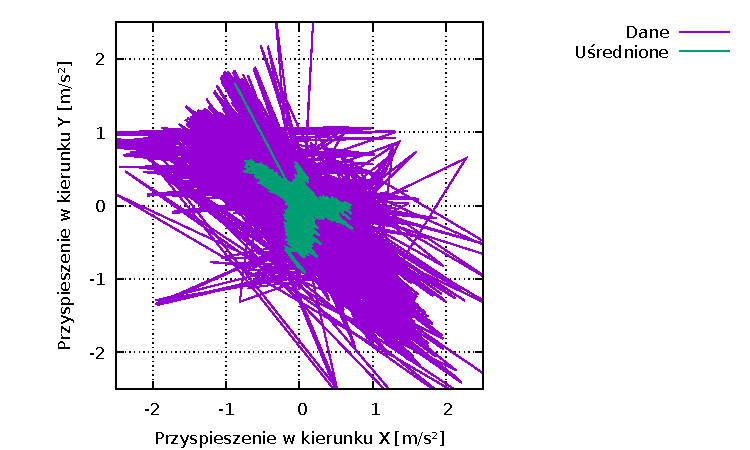
\includegraphics[width=\textwidth]{plots/wewucho_linear.pdf}
			\caption{Test przyspieszenia czujnika inercji.}
			\label{plot:wewucho_angular}
		\end{figure}
		
		Na czystych danych nie widać, jakoby model czujnika inercji w ogóle działał. 
		Jest to widoczne tylko przy natychmiastowej zmianie prędkości platformy, to jest przy teście \ref{sec:test_square}.
		Jednak takie teoretycznie nieskończone przyspieszenie nie może być w żaden naukowy sposób zinterpretowane, dlatego należy przeprowadzić testy z kontrolowanym
		przyspieszeniem.
		
		Po uśrednieniu danych z 10 ostatnich pomiarów, okazuje się, że środek generowanych w tym czasie danych jednak się przesuwał.
		Co więcej, robił to w poprawnych kierunkach.
		
		Na początku powstał zapis w kierunku dodatnim osi X, reprezentujący przyspieszenie platformy.
		Następnie program zanotował odchylenie pod kątem 45°, w drugiej kwadrze, co było nałożeniem się opóźnienia w osi X i przyspieszenia w osi Y.
		Na koniec zatrzymanie się platformy generowało zapis w ujemnym kierunku osi Y.
		
		Wykres generowany w czasie rzeczywistym sugeruje, jakoby niektóre pakiety przekazywały zerowe przyspieszenie, co w znaczącym stopniu wpływa na 
		ostatecznie generowane dane.
		
		Widać także, że wyraźnie zapisuje się tendencja danych do oscylowania na prostej pod kątem 45°.
		
		Akcelerometr platformy generuje bardzo podobne dane, które również są obarczone dużym błędem.
		Można powiedzieć zatem, że symulacja czujnika jest na dobrym poziomie.
		
		
		
		
		
	
	
